\section{Łukasz Garczyński}
\label{sec::garczynskil}

\subsection{Historia Polski}

\hspace{1cm} Polska historia to jak wędrówka przez burzliwe morze z licznymi wzlotami i upadkami. Zaczynamy od Mieszka I, który był jak pierwsza kropka na polskiej kartografii. Potem było trochę bitew, z czego jedna pod Grunwaldem, gdzie Polacy pokazali, że potrafią sobie radzić z dużymi sąsiadami.

\hspace{1cm} Potem trochę smutków związanych z rozbiorami, kiedy to Polska zniknęła z mapy na jakieś 123 lata. Ale wracamy do gry po I wojnie światowej i odzyskujemy niepodległość. Szybko jednak trzeba było stawić czoła kolejnej wojnie, która zaczęła się od dziwnej wyprawy niemieckiego konia wojennego przez nasze pola.

\subsection{Wyrażenie matematyczne}
\begin{equation}
     x = \frac{-b \pm \sqrt{b^2 - 4ac}}{2a}
\end{equation}

\subsection{Zdjęcie}

\vspace{0,5cm}
\begin{figure}[htbp]
\centering
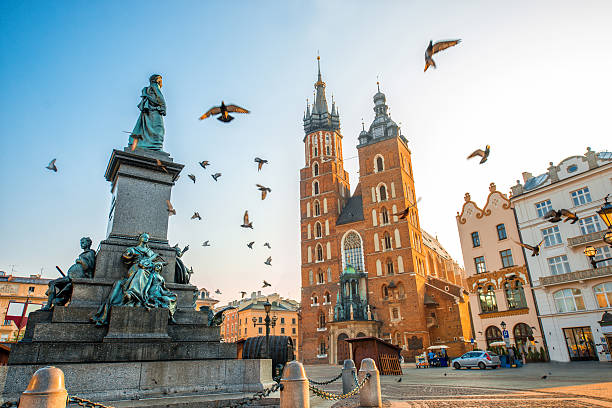
\includegraphics[scale=0.8]{pictures/krakow.jpeg}
\vspace{0,5cm}
\caption{Krakow}
\label{fig:krakow}
\end{figure}

\subsection{Największe polskie miasta}
\vspace{0,5cm}

\begin{table}[]
\begin{tabular}{|lll|}
\hline
\multicolumn{3}{|c|}{\textbf{Największe miasta w Polsce}}                                                                                                                     \\ \hline
\multicolumn{1}{|l|}{{\color[H \textit{\textbf{Lp.}}}} & \multicolumn{1}{l|}{{\color[HTML]{000000} \textit{\textbf{Miasto}}}} & {\color[HTML]{000000} \textit{\textbf{Liczba ludności}}} \\ \hline
\multicolumn{1}{|l|}{{\color[HTML]{000000} 1.}}                    & \multicolumn{1}{l|}{{\color[HTML]{000000} Warszawa}}                 & {\color[HTML]{000000} 1 861 975}                         \\ \hline
\multicolumn{1}{|l|}{{\color[HTML]{000000} 2.}}                    & \multicolumn{1}{l|}{{\color[HTML]{000000} Kraków}}                   & {\color[HTML]{000000} 803 283}                           \\ \hline
\multicolumn{1}{|l|}{{\color[HTML]{000000} 3.}}                    & \multicolumn{1}{l|}{{\color[HTML]{000000} Wrocław}}                  & {\color[HTML]{000000} 675 079}                           \\ \hline
\multicolumn{1}{|l|}{{\color[HTML]{000000} 4.}}                    & \multicolumn{1}{l|}{{\color[HTML]{000000} Łódź}}                     & {\color[HTML]{000000} 658 444}                           \\ \hline
\multicolumn{1}{|l|}{{\color[HTML]{000000} 5.}}                    & \multicolumn{1}{l|}{{\color[HTML]{000000} Poznań}}                   & {\color[HTML]{000000} 541 316}                           \\ \hline
\end{tabular}
\end{table}
\vspace{0,5cm}
Table ~\ref{tab:table6} 
\vspace{0,5cm}

\subsection{Przepis na zdrową owsiankę}
\vspace{0,5cm}
Składniki:
    \begin{itemize}
        \item 1/2 szklanki płatków owsianych
        \item 1 szklanka mleka (może być krowie, roślinne, np. migdałowe, sojowe)
        \item 1/2 szklanki wody
        \item Szczypta soli
        \item Opcjonalnie: miód, owoce, orzechy do dekoracji
    \end{itemize}
\vspace{0,5cm}

Instrukcje:
\begin{enumerate}
    \item W garnku połącz płatki owsiane, mleko, wodę i szczyptę soli.
    \item Podgrzewaj na średnim ogniu, często mieszając, aż owsianka zacznie się zagęszczać.
    \item Kiedy osiągnie odpowiednią konsystencję (po około 5-7 minutach), zdejmij z ognia.
    \item Przełóż owsiankę do miseczki i udekoruj według uznania. Możesz dodać miód, świeże owoce, orzechy, cynamon czy nasiona chia.
    \item Owsiankę podawaj ciepłą i gotową do spożycia!
\end{enumerate}
\vspace{0.5cm}


